%!TEX root = practicum2.tex
\begin{figure}%[b!]
	\centering
	\begin{subfigure}{0.45\columnwidth}
		\centering
		
\includegraphics[width=\textwidth]{img/assignment_connectivity_four_N80_p3.jpeg}
		\caption{4-connectivity}
		\label{fig:exp:connectivity:fourConnect}
	\end{subfigure}
	\begin{subfigure}{0.45\columnwidth}
		\centering
		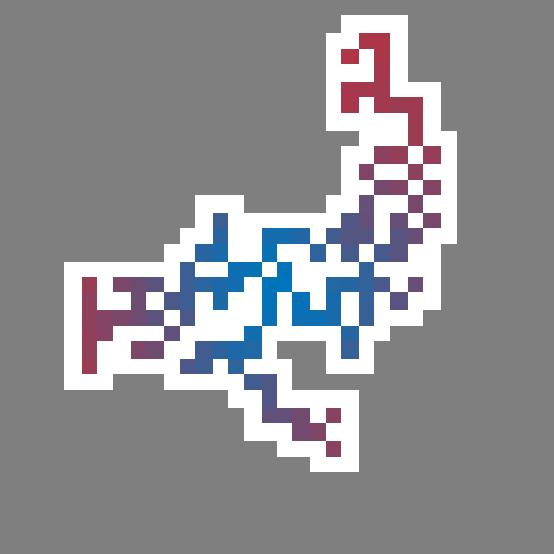
\includegraphics[width=\textwidth]{img/assignment_connectivity_eight_N80_p3.jpeg}
		\caption{8-connectivity}
		\label{fig:exp:connectivity:eightConnect}
	\end{subfigure}	
	\caption{The results of growing a cluster with the same grid of probabilites with \subref{fig:exp:connectivity:fourMask} four-connectivity and \subref{fig:exp:connectivity:eightMask} eight-connectivity. Note that although the clusters are generated on a grid with $N = 80$, we have plotted them on a grid with $N = 16$.}
	\label{fig:exp:connectivityResults}
\end{figure}

We consider two different connectivities, namely four- and eight-connectivity, which are illustrated in \cref{fig:exp:connectivity}. In this section we discuss the influence of the 8-connectivity on the size of the cluster.

\Cref{fig:exp:connectivityResults} shows two clusters which have been grown using the same probabilities but different connectivities. We see that in this case the 8-connected cluster is much larger than the 4-connected cluster. Although a different seed for the algorithms may result in different clusters in general one would expect the 8-connected cluster to grow larger than the 4-connected version. Since the expected number of sites that are occupied in each grow step when 8-connectivity is used is twice as high as the expected number of occupied sites with 4-connectivity. 

% Influence of probability
The results of performing the same experiment as discussed in \cref{ss:exp:probability} with the eight-connectivity mask, are presented in \cref{fig:experiment:conn:mean_std_clusters} in \cref{ap:ss:Connectivity} and \cref{fig:experiment:conn:p_inf_ratio}. We have changed the range of $p$ to $p = 0.2, 0.21, \dotsc, 0.6$, since even for $p = 0.3$ $P_\infty$ was close to zero. 

\begin{figure}%[b!]
	\centering
	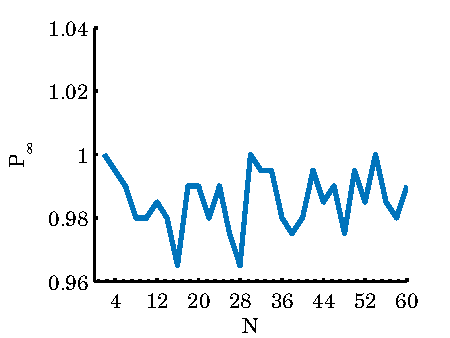
\includegraphics[width=\columnwidth]{./img/assignment_d_p_infinite_ratio_p.pdf}
	\caption{Ratio of percolating clusters, $P_\infty$, as a function of $p = 0.2, 0.21, \dotsc, 0.6$ when eight-connectivity is used. Ratios are calculated over $r_{max} = 200$ runs on a $41 \times 41$ grid.}
	\label{fig:experiment:conn:p_inf_ratio}
\end{figure}

% \begin{figure*}
% 	\centering
% 	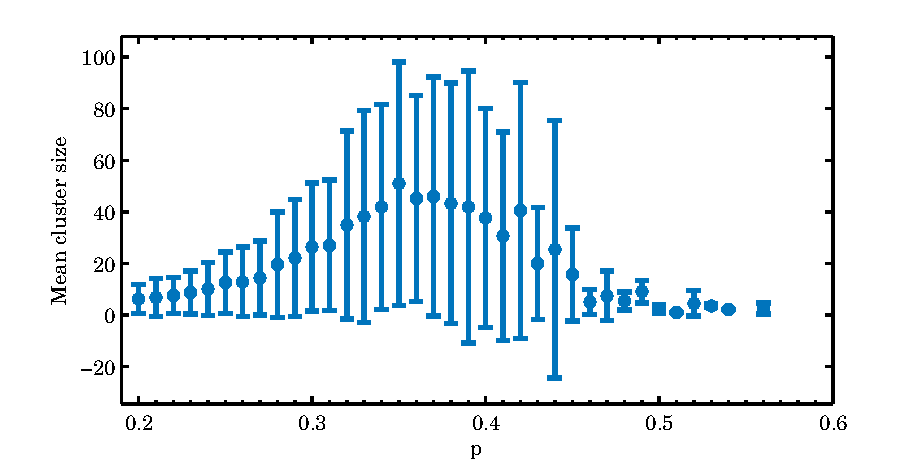
\includegraphics[width=\textwidth]{./img/assignment_d_mean_std_p.pdf}
% 	\caption{Mean cluster sizes, represented as points, and standard deviations, indicated by the vertical error bars, as a function of $p = 0.2, 0.21, \dotsc, 0.6$ when eight-connectivity is used. The mean and standard deviation were calculated over $200$ runs on a $41 \times 41$ grid.}
% 	\label{fig:experiment:conn:mean_std_clusters}
% \end{figure*}

It should be noted that for some values of $p$, especially larger values there are no mean cluster sizes, since no finite clusters were found. This indicates that one is much more likely to encounter a percolating cluster with eight-connectivity than with four-connectivity for the same value of $p$. Which fits with our ealier observation that the expected number of newly occupied sites with eight-connectivity is twice as high when compared with a four-connected cluster.

That for higher values of $p$ a percolating cluster is more likely than a finite cluster is confirmed by \cref{fig:experiment:conn:p_inf_ratio}, where we find that only for very low values of $p$ $P_\infty$ is zero, and that $P_\infty$ quickly approaches 1. 

These findings suggest that $p_c$ is much lower when eight-connectivity is used. Based on this, admittedly small experiment, one would guess $p_c$ to be approximately $0.2$ when eight-connectivity is used. More research is needed to find the actual value of $p_c$ for eight-connected clusters.\\


% \todo{Influence of size}
% % To determine the influence of the connectivity on the size we have performed the same experiment as used for the four-connectivity. \todo[inline]{Resultaten}

% \todo{Influence on fractal dimension}
% % We have determined the fractal dimension of the cluster generated using four connectivity for $N = 80$ and $p =0.7$. We have found that \todo[inline]{Resulaten}

